\documentclass[12pt]{report}
\usepackage{pgfplots}

\pgfplotsset{
	curve plot style/.style={
		xlabel={N - Number of top database candidates},
		xmin=0, xmax=25,
		xtick={0,5,10,15,20,25},
		ytick={45,50,55,60,65,70,75,80,85,90,95,100},
		legend pos=south east,
		ymajorgrids=true,     xmajorgrids=true,
		grid style=dashed,
		ylabel={Recall@N (\%)},
		ylabel style={yshift=-.3cm},
		width=8.5cm,
		height=10cm,
	},
}


\usepackage[margin=0.5in]{geometry}
\usepackage[utf8]{inputenc}
\usepackage{epsfig} %
\usepackage{ tipa }
\usepackage{ textcomp }
\usepackage{float}
\usepackage{ dsfont }
\usepackage{multirow}
\usepackage{ltablex}
\usepackage{siunitx}
\usepackage{subfloat}
\usepackage{pdfpages}
\usepackage{moreverb,url}
\sisetup{table-format=-2.0, table-number-alignment=center}
\usepackage[colorlinks,bookmarksopen,bookmarksnumbered,citecolor=red,urlcolor=red]{hyperref}
\usepackage[ruled,vlined,noresetcount]{algorithm2e}
\usepackage[noend]{algpseudocode}
\usepackage[
font=footnotesize %
]{subfig}

\usepackage{cite}
\usepackage{amsmath,amssymb,amsfonts}
\usepackage{graphicx}
\usepackage{textcomp}
\usepackage{xcolor}
\SetKwFunction{KwFn}{Fn}
\SetKwProg{Fn}{Function}{}{}
\linespread{1.5}

\setlength{\topmargin}{-0.5cm}
\setlength{\textheight}{23.5cm}
\setlength{\oddsidemargin}{1.5cm}
\setlength{\evensidemargin}{0cm}
\setlength{\textwidth}{14.4cm}
\setlength{\headsep}{0in}
\setlength{\parskip}{.15in}
\setlength{\parindent}{0in}

\usepackage{setspace} %

\usepackage{nomencl}
\makenomenclature
\renewcommand{\nomname}{ABBREVIATIONS}

\definecolor{Mycolor2}{HTML}{1560BD}
\newcommand{\colorit}[1]{{\color{Mycolor2}{#1}}}
\usepackage{xcolor}
\definecolor{mediumBlue}{rgb}{0.15,0.15,0.75}
\definecolor{darkBlue}{rgb}{0,0,0.5}


\usepackage{float}
\usepackage{tikz,xcolor}
\usepackage{xcolor}
\usepackage{tcolorbox}

\usepackage{bibentry}
\usepackage[numbers,sort&compress,sectionbib]{natbib}
\usepackage{chapterbib}

\bibliographystyle{ieeetr}



\newcommand{\thesisWriter}{Muhammad Usman Maqbool Bhutta}

\begin{document}

\pagenumbering{roman}

\addcontentsline{toc}{chapter}{Title Page}

\null\vspace{0.5in}
\begin{center}
{\Large\bf Towards a Swift Multiagent SLAM System for Large-Scale Robotics Applications}
\vspace{2.5cm}

{\large by}
\vspace{0.5cm}

{\large\bf \thesisWriter{}}\normalsize
\vspace{2.5cm}

A Thesis Submitted to \\
The Hong Kong University of Science and Technology \\
in Partial Fulfillment of the Requirements for \\
the Degree of Doctor of Philosophy \\
in the Department of Electronic and Computer Engineering
\vspace{1.5cm}

February 2021, Hong Kong
\end{center}

\newpage

\addcontentsline{toc}{chapter}{Authorization Page}
\begin{center}{\Large\bf Authorization}\normalsize
\end{center}
\vspace{0.5cm}

I hereby declare that I am the sole author of the thesis.

\vspace{0.5cm}

I authorize the Hong Kong University of Science and Technology to lend this thesis
to other institutions or individuals for the purpose of scholarly research.

\vspace{0.5cm}

I further authorize the Hong Kong University of Science and Technology to
reproduce the thesis by photocopying or by other means, in total or in
part, at the request of other institutions or individuals for the
purpose of scholarly research.

\vspace{0.3cm}

\begin{figure}[h]
	\centering
	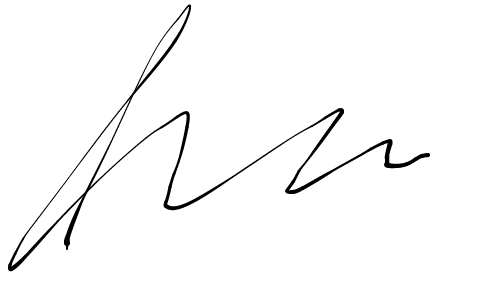
\includegraphics[scale=.20]{includes/sig.png}
\end{figure}
\begin{center}
\vspace*{-1.7cm}
\line(1,0){180}
\smallskip

\thesisWriter{}

February 2021
\end{center}

\newpage

\addcontentsline{toc}{chapter}{Signature Page}
\null\vspace{0.4cm}
\begin{center}
{\Large\bf Towards a Swift Multiagent SLAM System for Large-Scale Robotics Applications}
\vspace{0.5cm}

{\large by}\smallskip

{\large\bf Muhammad Usman Maqbool Bhutta}\normalsize

\vspace{0.5cm}

This is to certify that I have examined the above PhD thesis and have found that it is complete and satisfactory in all respects, and that any and all revisions required by the thesis examination committee have been made.

\vspace{0.4cm}

\line(1,0){230} 

Professor Ming Liu (ECE), Thesis Supervisor

\vspace{0.4cm}

\line(1,0){230} 

Professor Bertram Emil Shi (ECE), Head of ECE Department

\begin{flushleft}
\textbf{Thesis Examination Committee} \vspace{0.1cm}
\begin{table}[H]
	\renewcommand{\arraystretch}{1.1}
    \begin{tabular}{ll}
	1. Professor Ming Liu & \multirow{2}{*}{Department of Electronic and Computer Engineering}\\
	\quad(Thesis Supervisor) & ~  \\
    2. Professor Wei Zhang & Department of Electronic and Computer Engineering\\
    3. Professor Yiwen Wang & Department of Electronic and Computer Engineering\\
    4. Professor Qiong Luo & Department of Computer Science \& Engineering\\
    5. Professor Xiong Rong & College of Control Science and Engineering,\\
    \quad(External Examiner) & Zhejiang University, Hangzhou, Zhejiang, China. 
    \end{tabular}
\end{table}
\end{flushleft}
Department of Electronic and Computer Engineering \\
The Hong Kong University of Science and Technology \\
February 2021
\end{center}


\newpage

\addcontentsline{toc}{chapter}{Acknowledgments}
\begin{center}{\Large\bf Acknowledgment}\normalsize
\end{center}
\vspace{0.5cm}

I would like to express my deep gratitude to my supervisor, Prof. Ming Liu who has given me a lot of advice and kindly support in my research during the years of my PhD study. I would like to thank The Punjab Educational Endowment Fund (PEEF) for providing me with the CMMS PhD scholarship award so I had the valuable opportunity to study here. This thesis and the work it embodies would not have been possible without the continual support of a number of individuals and organizations. I would like to take this opportunity to express my gratitude to everyone who has contributed to the fulfillment of this thesis. I want to gratefully acknowledge and express my appreciation to my supervisor, Prof. Ming Liu, for his invaluable guidance, full support and patience through my PhD studies. His outstanding attributes such as humility, diligence, enthusiasm and dedication, together with his amazing academic insights and on-going belief were constant sources of motivation for me. I am truly privileged to have had him as my supervisor. I would like to thank Prof. Roland Siegwart and Dr. Cesar Dario Cadena Lerma from the Autonomous Systems Lab, ETH Zürich, Switzerland for kindly welcoming me to visit their research group. The discussions with them stimulated many interesting ideas in my research area of place recognition. Thanks must go to The Hong Kong University of Science and Technology for providing the top up support to my PhD scholarship and overseas research scholarship along with a wealth of other supports during the most painful time of my life. It has been my great pleasure to carry out my PhD study in the RAM-LAB @ HKUST research group. I would like to thank everyone for making it friendly and providing desirable environment for research discussions. Special thanks should be given to the staff in the department administration for all their assistance and patience. I am deeply thankful to my amazing parents and for the way they raised me, without which it would be impossible to be who I am at the moment. Last, I would like to dedicate this thesis and everything I do to my love, who is always with me.

\newpage
\thispagestyle{empty}
\null\vskip0.5in
\begin{center}


  \vspace{20mm}

  \begin{LARGE}
    \textit{To my family...}
  \end{LARGE}

  \vspace{4mm}



\end{center}

\vfill

\newpage

\addcontentsline{toc}{chapter}{Table of Contents}

\begin{spacing}{0.25}
   {\footnotesize \tableofcontents}
\end{spacing}

\newpage
\addcontentsline{toc}{chapter}{List of Figures}
\listoffigures

\newpage
\addcontentsline{toc}{chapter}{List of Tables}
\listoftables


\newpage


\newpage
\addcontentsline{toc}{chapter}{Abbreviations}
\printnomenclature[1in]

\newpage
\pagenumbering{arabic}



\addcontentsline{toc}{chapter}{Abstract}
\begin{center}
{\Large\bf Towards a Swift Multiagent SLAM System for Large-Scale Robotics Applications}
\vspace{0.5cm}

{\large \bf \thesisWriter{}}\normalsize

\medskip

Department of Electronic and Computer Engineering\\ The Hong Kong University of Science and Technology

\end{center}
\vspace{1.5cm}
\centerline{{\bf \large Abstract}}
\vspace{1.5cm}

Abstract goes here.













\chapter{Introduction}\label{ch1-intro}

\section{Introduction-1}

\section{Introduction-2}

\section{Introduction-3}

\section{Thesis Contributions}
Some text... \\

\subsection{Contribution 1: TITLE}
Some text...
Our contributions are as follows:\\
\begin{itemize}
	\item Some text....
	\item We introduce Some text....
	\item Some text....
	\item Some text....
\end{itemize}  
\subsection{Contribution 2: TITLE}
Some text...
Our contributions include:\\
\begin{itemize}
	\item Some text...
	\item Some text...
	\item Some text...
	\item Some text...
\end{itemize} 
\subsection{Contribution 3: TITLE}
Some text... The contribution of this research is four-fold, as follows:\\
\begin{itemize}
	\item Some text...
	\item Some text...	
	\item Some text... 
	\item Some text... 
\end{itemize}
\section{Thesis Overview}
The remainder of this thesis is organized as follows. Chapter ... \\
\section{Publications}
\addcontentsline{toc}{chapter}{List of Publications}
\nobibliography*
\subsection{Journal Papers}
\begin{itemize}
	\item \bibentry{bhutta2020loopbox}.
	\item \bibentry{maqbool}.
\end{itemize}

\subsection{Conference Papers}
\begin{itemize}
	\item \bibentry{Bhutta2018}.
\end{itemize}
\subsection{Other Publications during Study}
\begin{itemize}
	\item \bibentry{bhutta2020}.
	\item \bibentry{bhutta2018b}.
\end{itemize}
\section{Related Material and Demo Videos}
\begin{itemize}
\item ``PCR-Pro'': \href{https://sites.google.com/view/pcr-pro}{https://sites.google.com/view/pcr-pro}.
\item ``Loop-Box'': \href{https://usmanmaqbool.github.io/loop-box}{https://usmanmaqbool.github.io/loop-box}.
\item ``MAQBOOL'': \href{https://usmanmaqbool.github.io/why-so-deep}{https://usmanmaqbool.github.io/why-so-deep}.
\item ``Smart-Inspect": \href{https://usmanmaqbool.github.io/smart-inspect}{https://usmanmaqbool.github.io/smart-inspect}.	
\end{itemize}
\newpage
\renewcommand*{\bibname}{\section{References}}%
\bibliographystyle{ieeetr}
\bibliography{Thesis}	
\chapter{Scientific Background and Literature Review}\label{sec-related-works}


This chapter includes all your thesis literature review.



\section{SLAM}
\label{chapter_2_slam}



\subsection{Graph SLAM}
\label{chapter_2_g_slam}
. 

\Section{Bundle Adjustment}
\label{chapter_2_ba}



\newpage
\renewcommand*{\bibname}{\section{References}}%
\bibliographystyle{ieeetr}
\bibliography{Thesis}		


\chapter{Figures}
\label{sec-pcr-pro}

\section{Single Image Configuration}
Use can use pdf image as well.
\begin{figure}[!h]
	\centering
	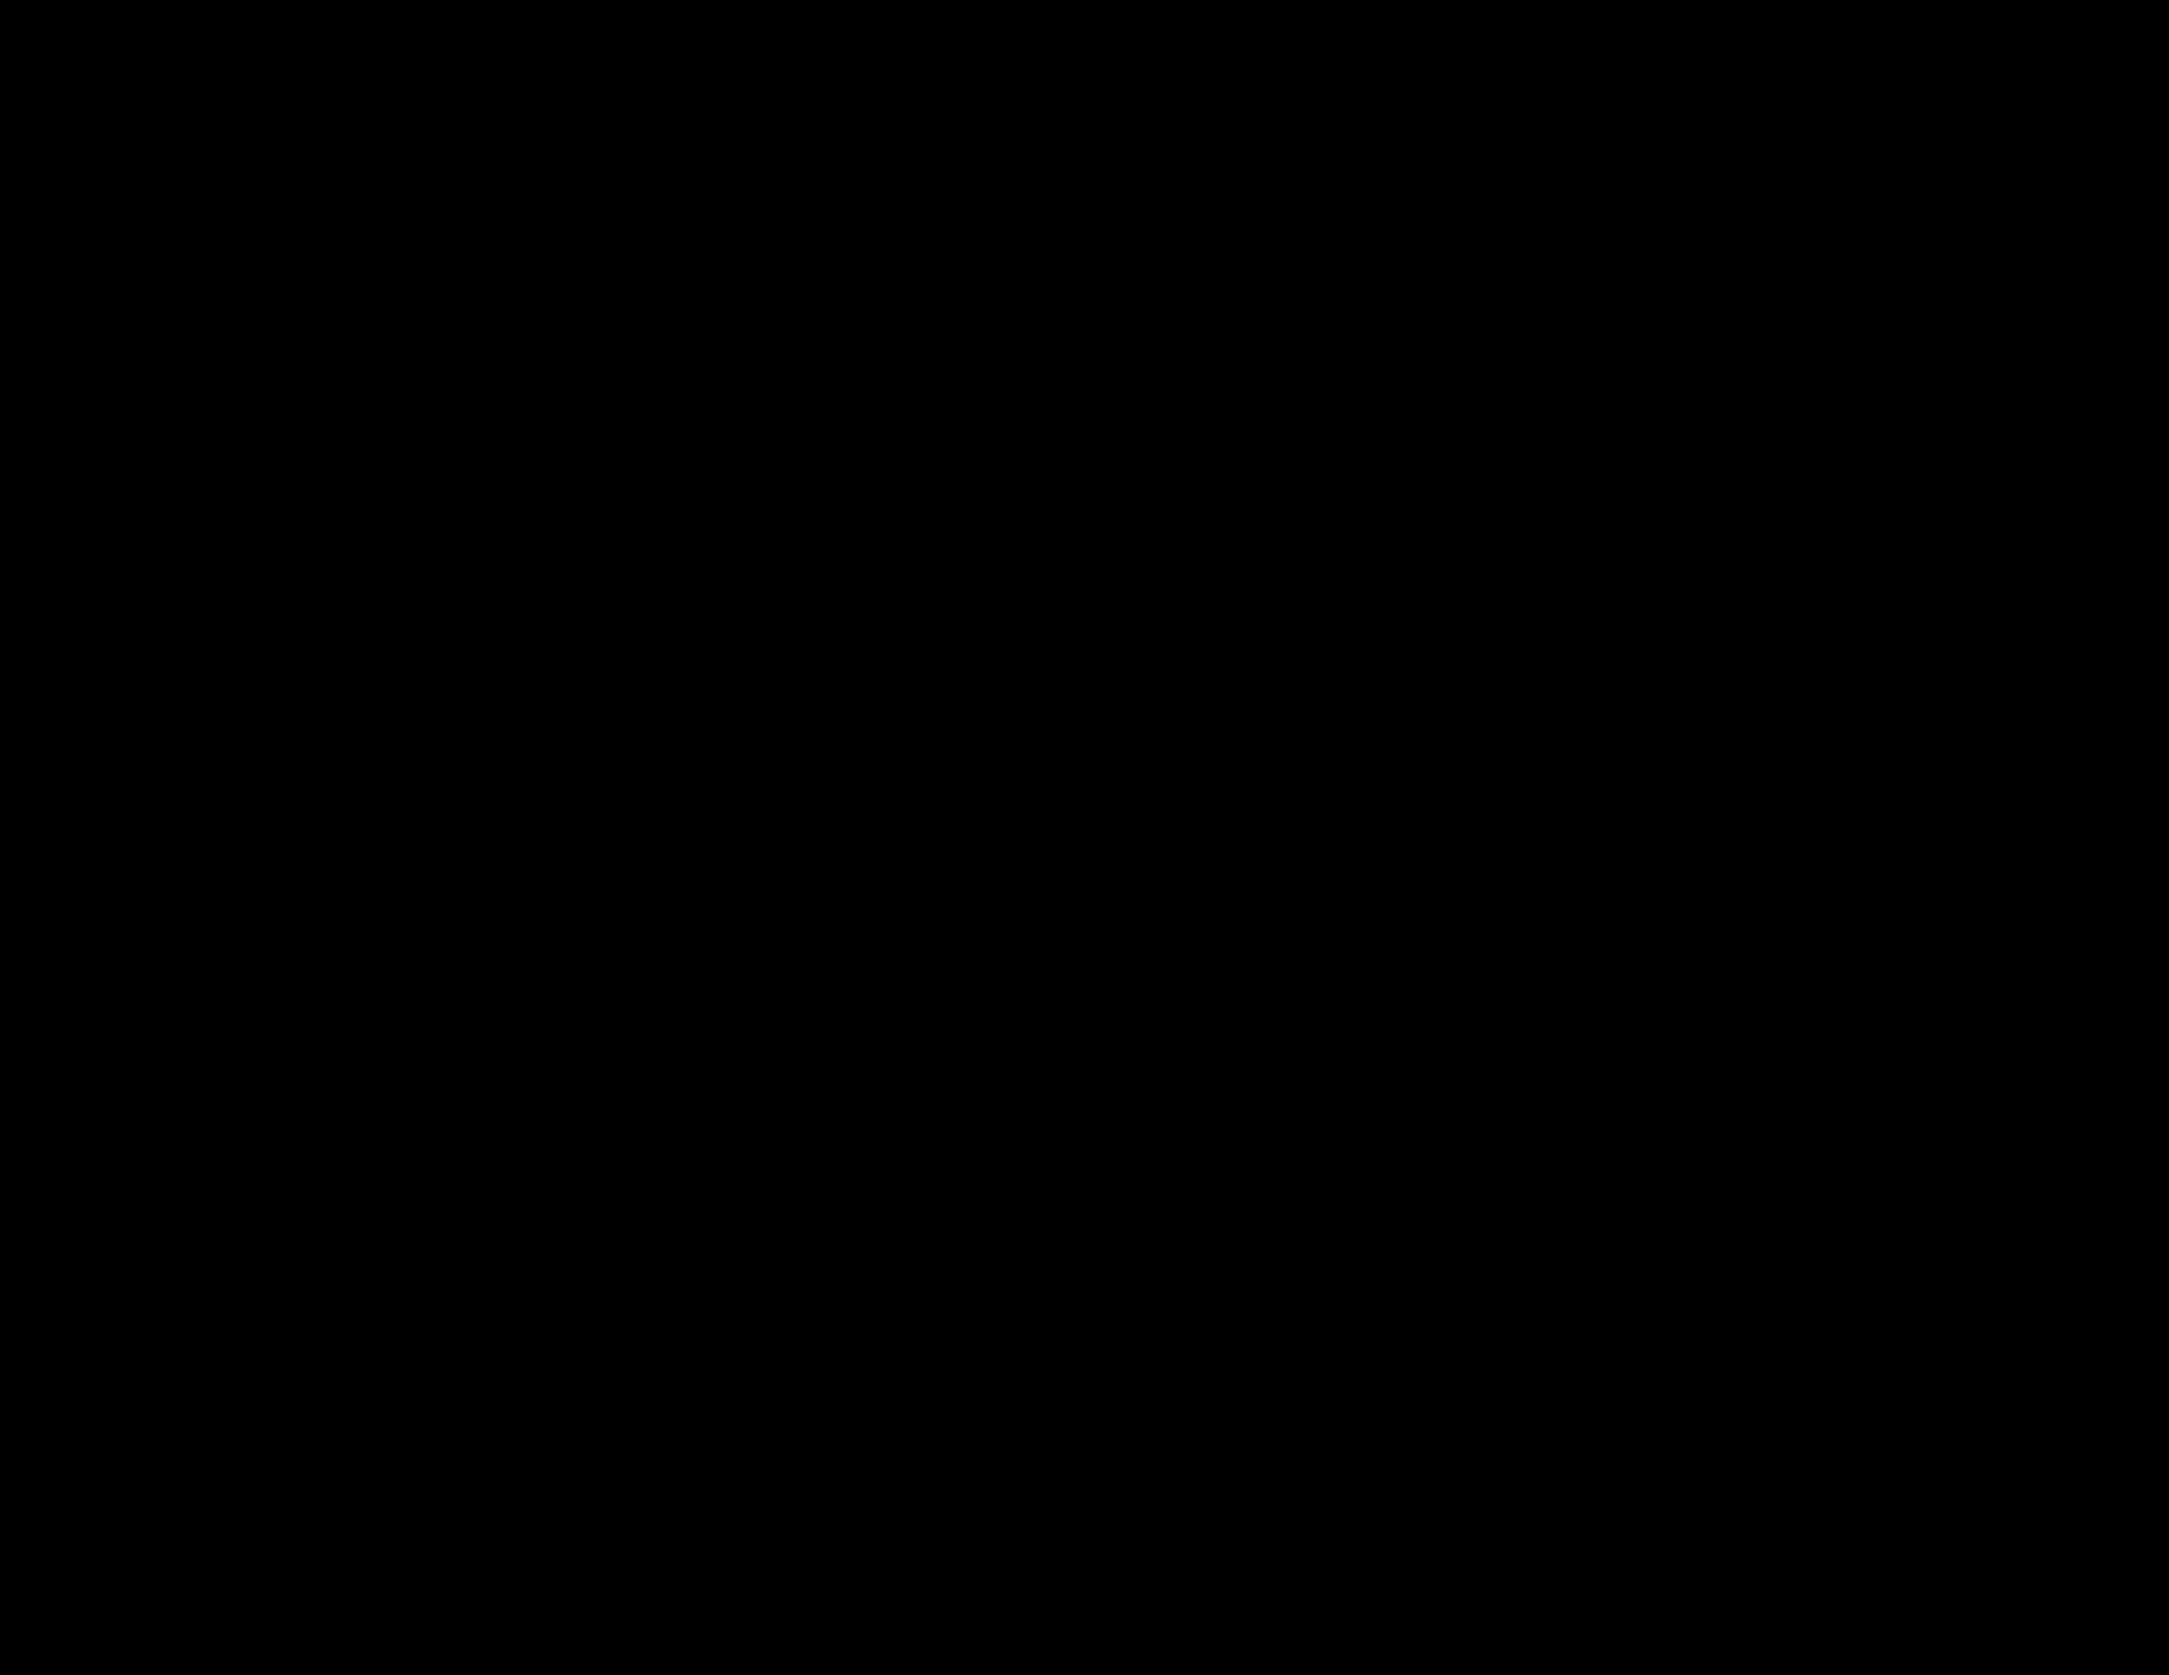
\includegraphics[width=.9\linewidth]{pdf/Result.pdf}
	\caption{Single Image Configuration.}
	\label{fig:single_image_Configuration}
\end{figure}

\newpage
\section{1-1 Configuration}

\begin{figure*}[!h] 
	
	\captionsetup[subfigure]{width=.9\linewidth}
	\subfloat[First Image] {\label{fig:1_1_Configuration_1} 
		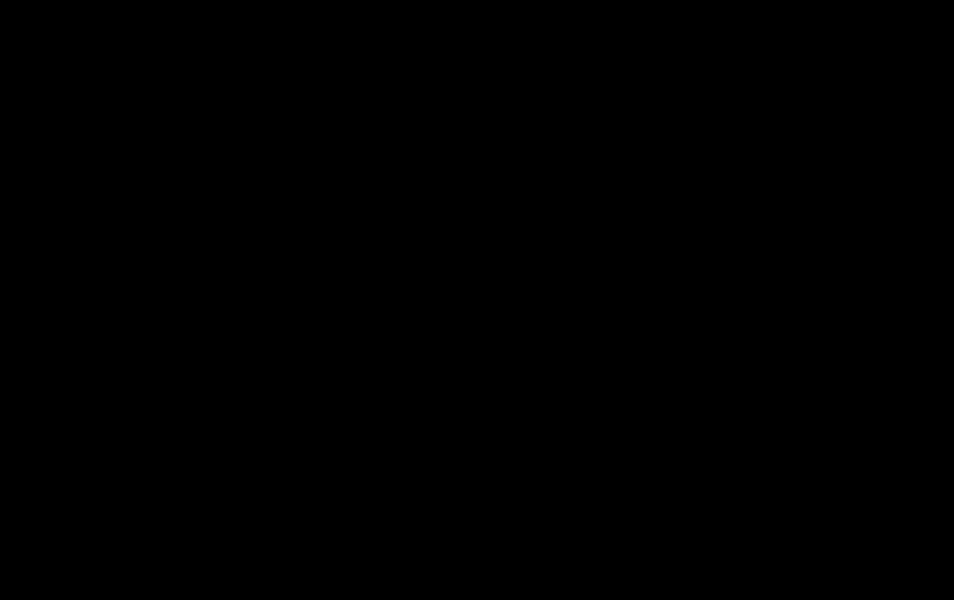
\includegraphics[width=.9\linewidth]{images/std.jpg}
		
	}
	\captionsetup[subfigure]{width=.9\linewidth}
	\subfloat[Second Image.] {\label{fig:1_1_Configuration_2}
		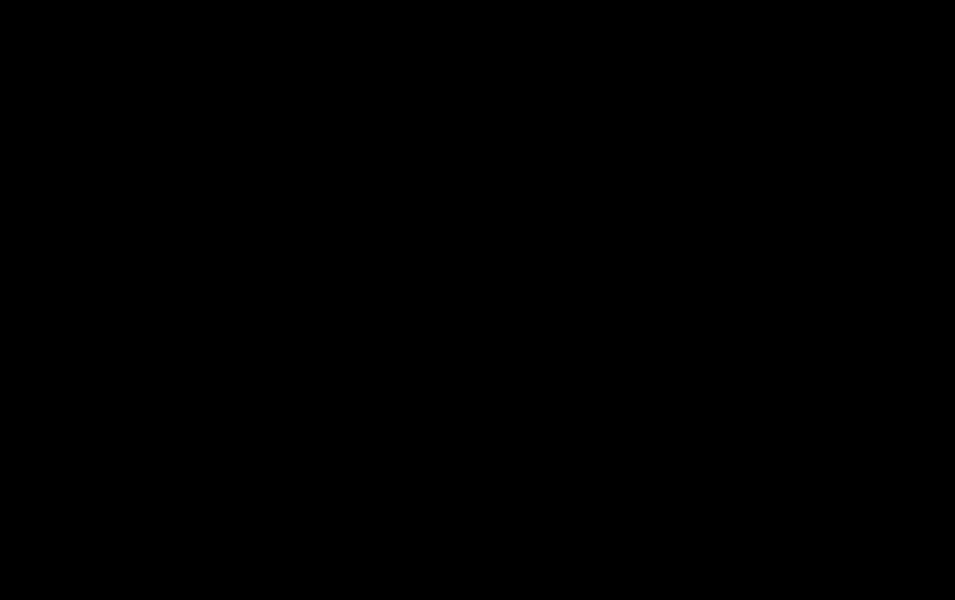
\includegraphics[width=.9\linewidth]{images/std_pcr_pro.jpg}
	}
	\caption{1-1 Configuration.}
	\label{fig:1_1_Configuration} 
\end{figure*}

\newpage
\section{2-1 Configuration}

\begin{figure}[!h] 
	\captionsetup[subfigure]{width=.48\linewidth}
	\subfloat[Image A.]{\label{fig:2_1_Configuration_1}
		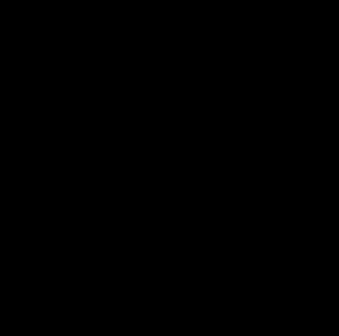
\includegraphics[width=.48\linewidth]{images/Result1/original_poses.jpg}
	}
	\subfloat[Image B.]{\label{fig:2_1_Configuration_2}
		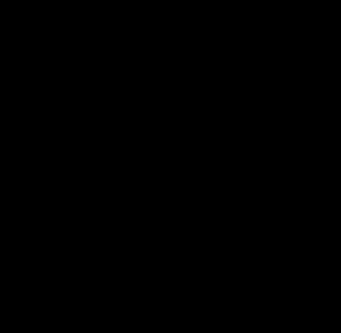
\includegraphics[width=.48\linewidth]{images/Result1/slam.jpg}
	} \\
	\captionsetup[subfigure]{width=.95\linewidth}
	\subfloat[Image C.]{\label{fig:2_1_Configuration_3}
		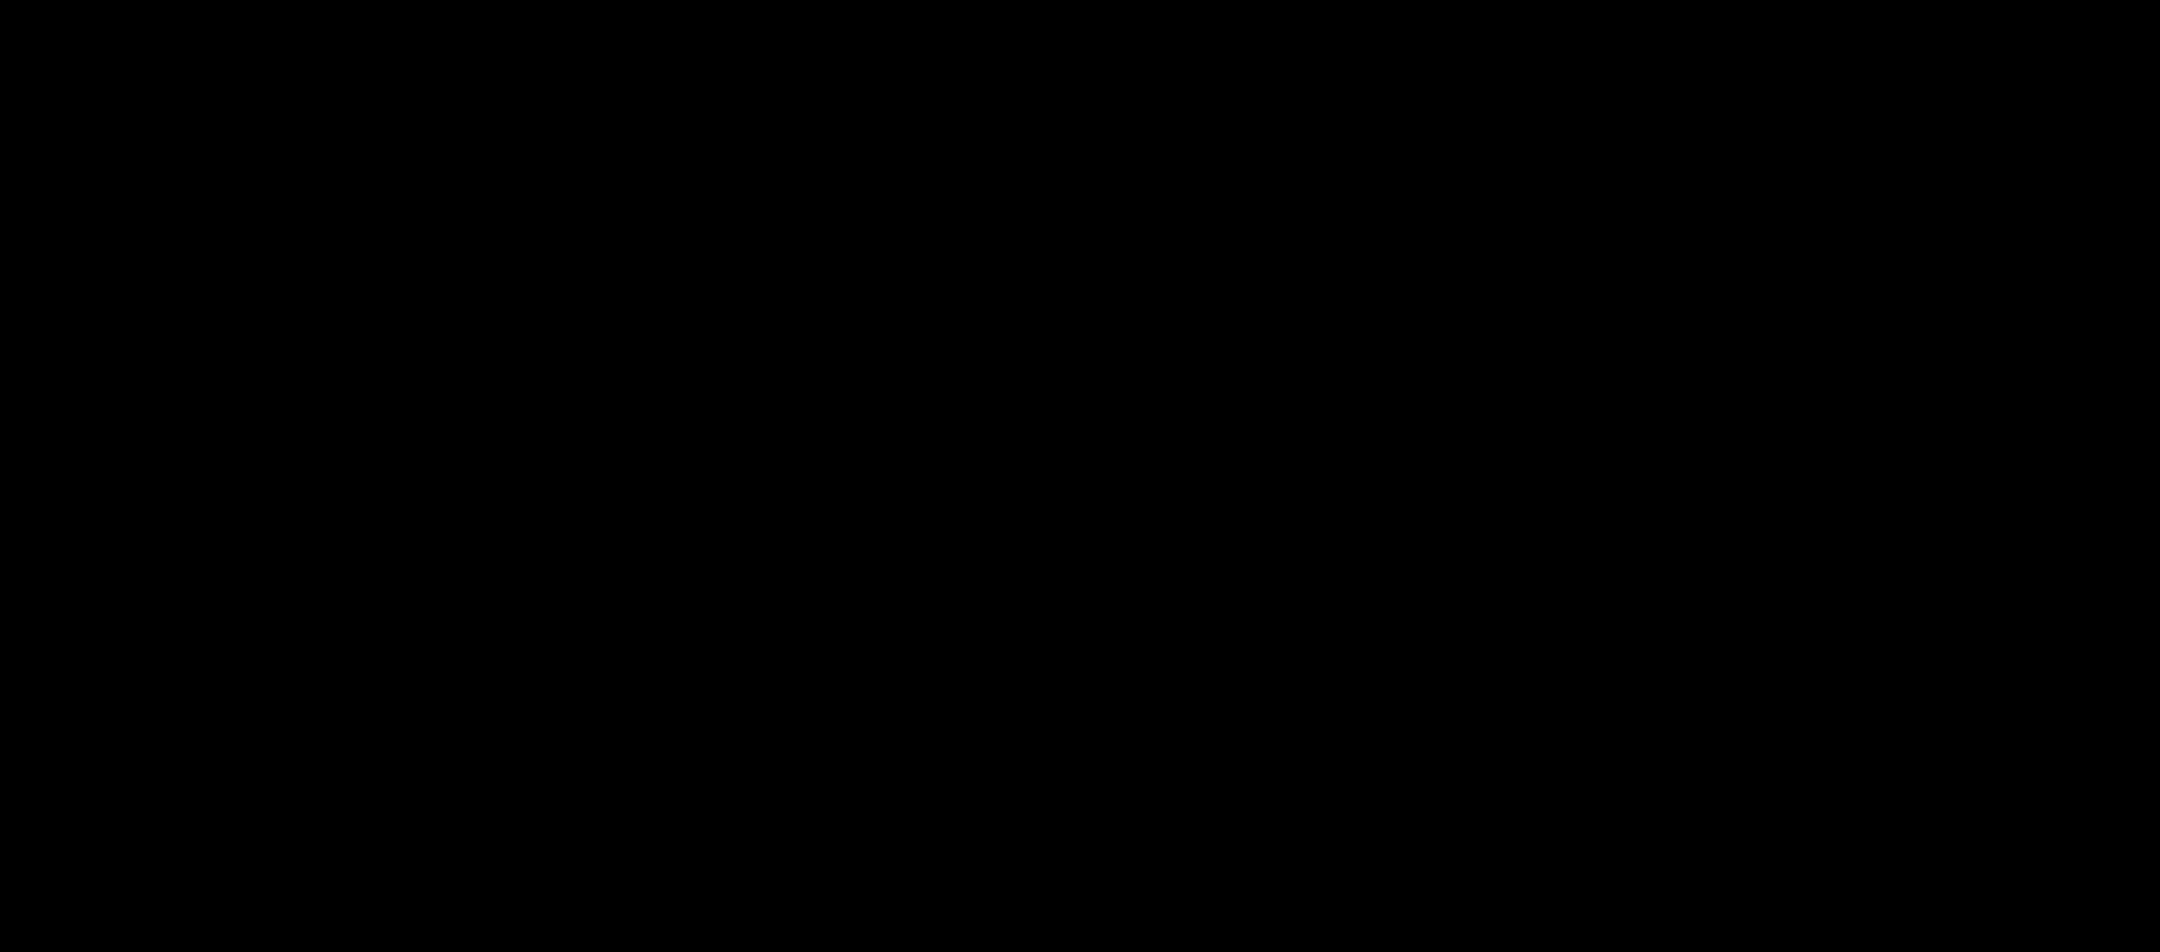
\includegraphics[width=.98\linewidth]{images/Result1/fullview.jpg}
	}
	\caption{2-1 Configuration.}
	\label{fig:2_1_Configuration} 
\end{figure}
\newpage
\section{4 x 4 Configuration}
\begin{figure}[!h] 
	\captionsetup[subfigure]{width=.45\linewidth}
	
	\subfloat[Image 21.]{\label{fig:4_4_Configuration_1}
		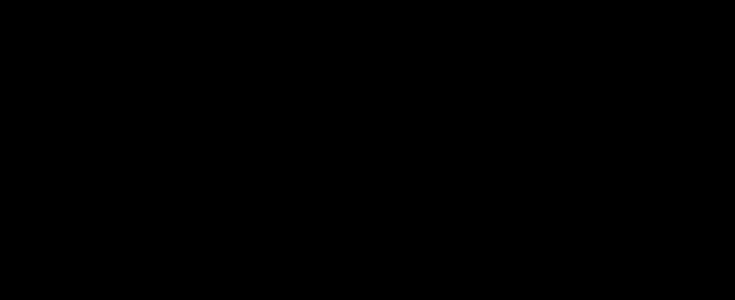
\includegraphics[width=.45\linewidth]{images/fig21.jpg}
	}
	\subfloat[Image 23.]{\label{fig:4_4_Configuration_2}
		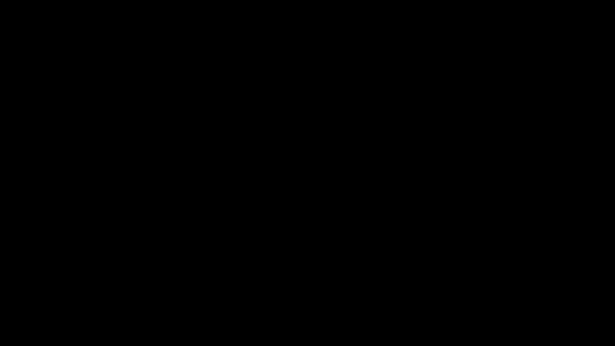
\includegraphics[width=.45\linewidth]{images/fig23.jpg}
	} \\
	\subfloat[Image 22.]{\label{fig:4_4_Configuration_3}
		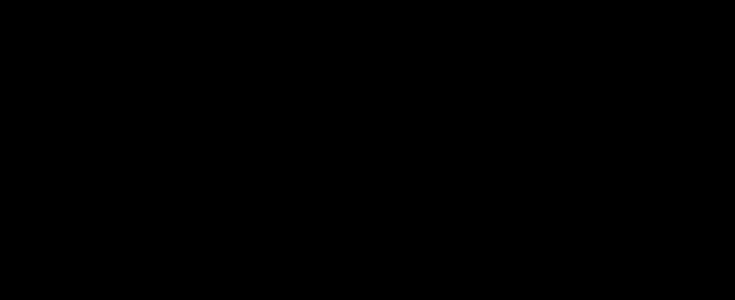
\includegraphics[width=.45\linewidth]{images/fig22.jpg}
	}
	\subfloat[Image 24.]{\label{fig:4_4_Configuration_4}
		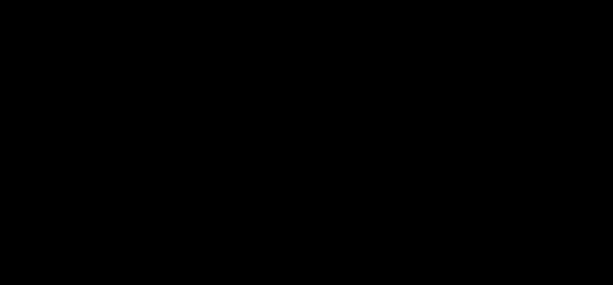
\includegraphics[width=.45\linewidth]{images/fig24.jpg}
	}
	
	\caption{4 x 4 Configuration.}
	\label{fig:4_4_Configuration} 
\end{figure}


\newpage
\section{3 x 2 Configuration}
\begin{figure*}[!h] 
	\centering
	
	\captionsetup[subfigure]{width=.32\linewidth}
	\subfloat[Image 1.]{\label{fig:3_2_Configuration_a}
		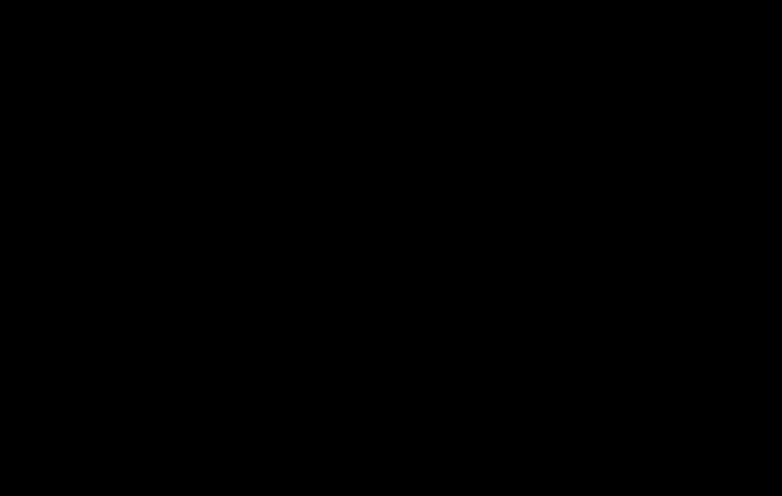
\includegraphics[width=.32\linewidth]{images/Result3/bundle_three_odom_threepoint_ueye5_ueye6.jpg}
	}
	\subfloat[Image 2.]{\label{fig:3_2_Configuration_b}
		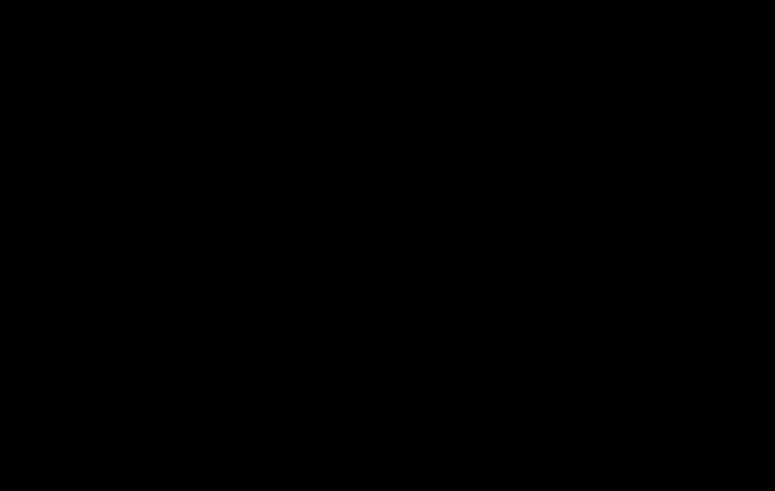
\includegraphics[width=.32\linewidth]{images/Result3/loop_box_three_odom_threepoint_ueye5_ueye6.jpg}
	}
	\subfloat[Image 3.]{\label{fig_loop_box_pgo_parking2_c}
		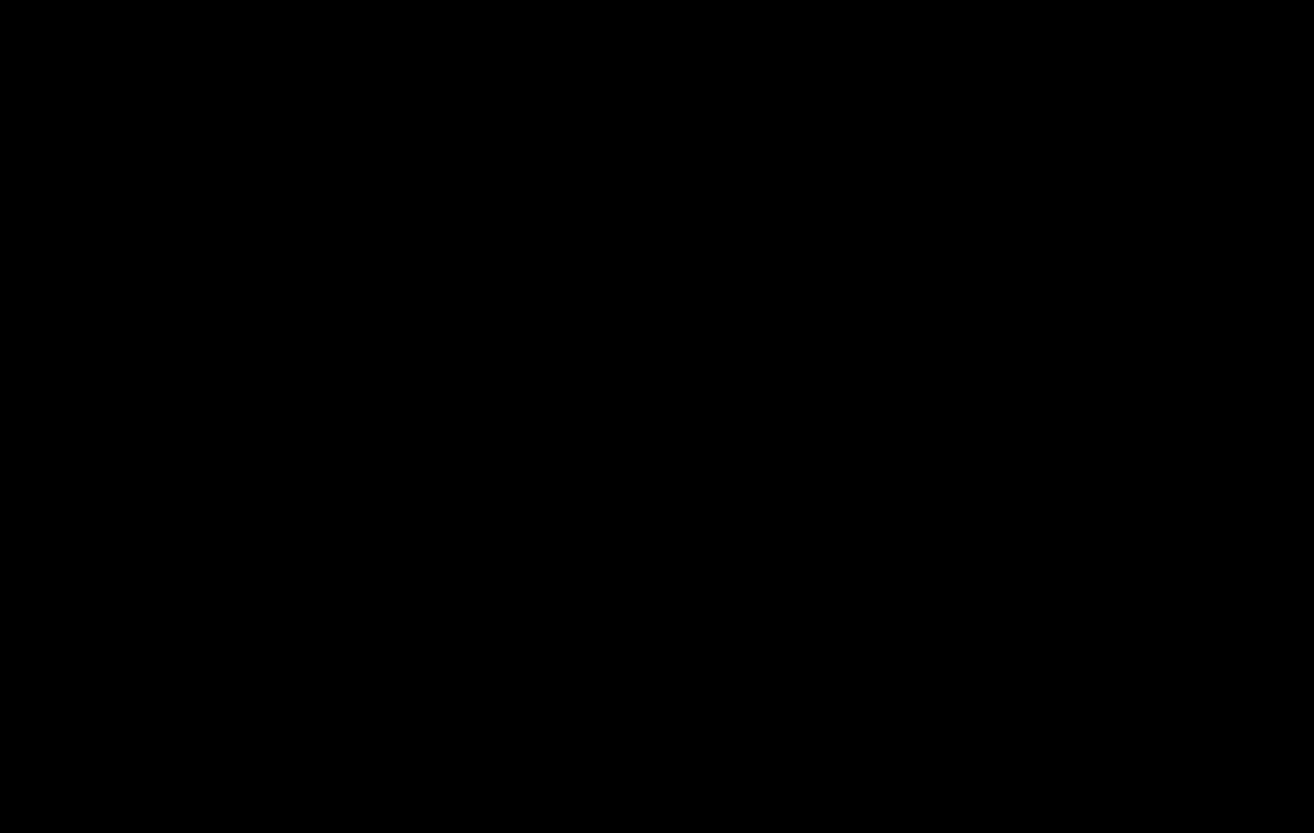
\includegraphics[width=.32\linewidth]{images/Result3/full_odom.jpg}
	}\hfil
	\subfloat[Image 4.]{\label{fig:3_2_Configuration_d}
		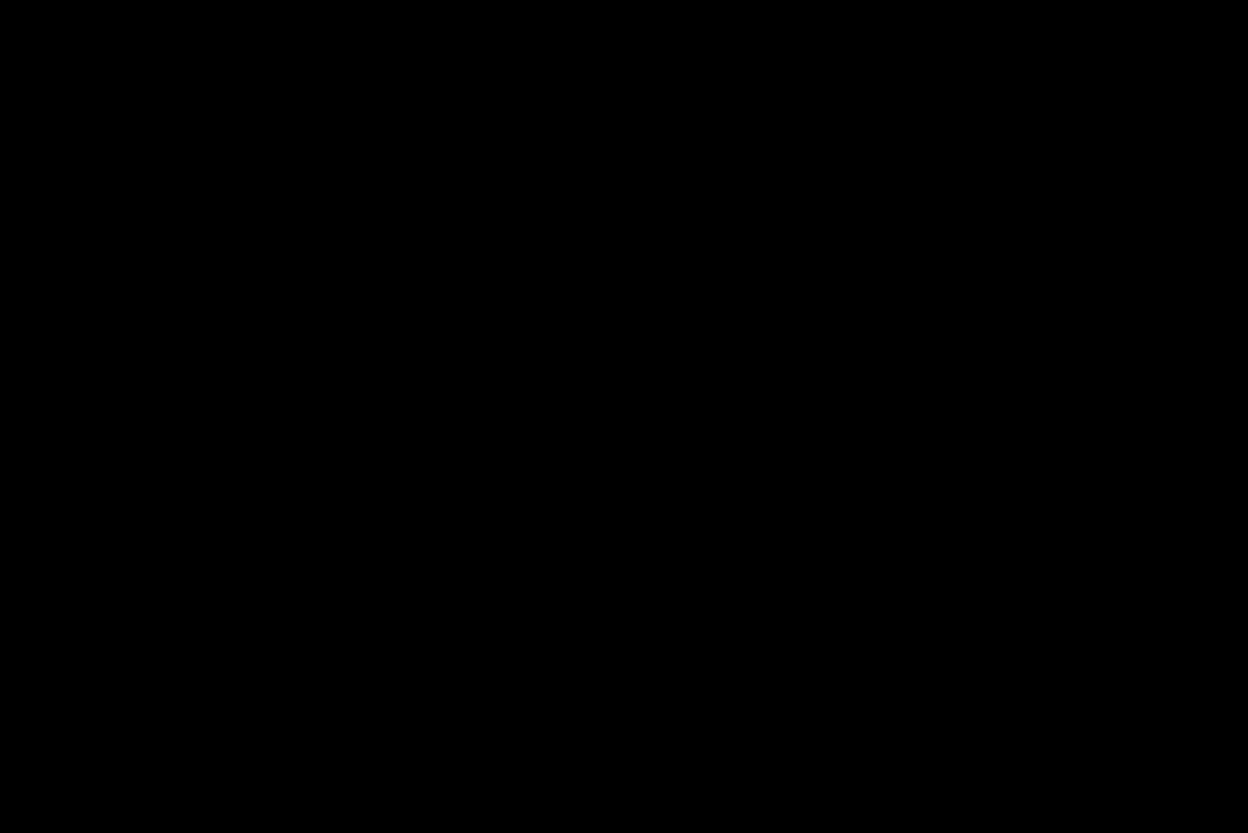
\includegraphics[width=.32\linewidth]{images/Result4/bundle_three_odom_threepoint_ueye5_ueye6.jpg}
	}
	\subfloat[Image 5.]{\label{fig:3_2_Configuration_e}
		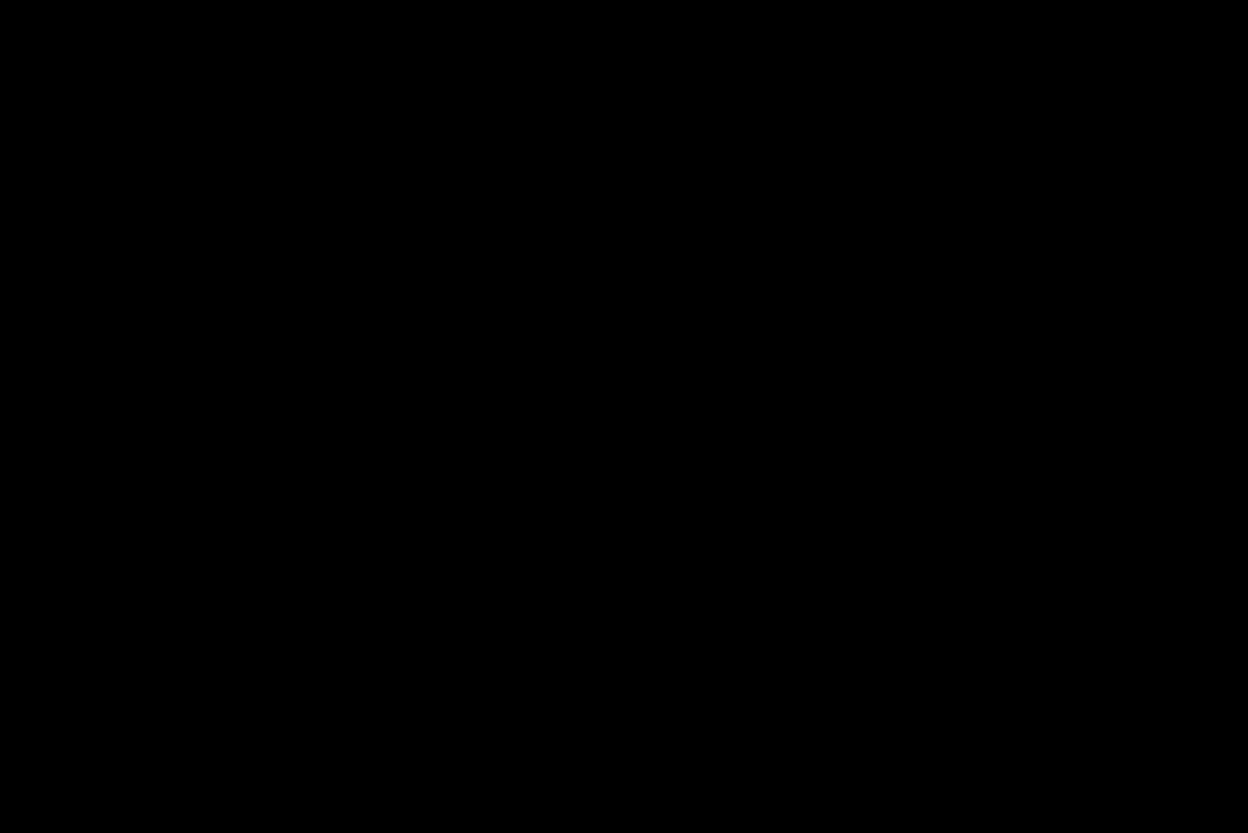
\includegraphics[width=.32\linewidth]{images/Result4/loop_box_three_odom_threepoint_ueye5_ueye6.jpg}
	}
	\subfloat[Image 6.]{\label{fig_loop_box_pgo_parking2_f}
		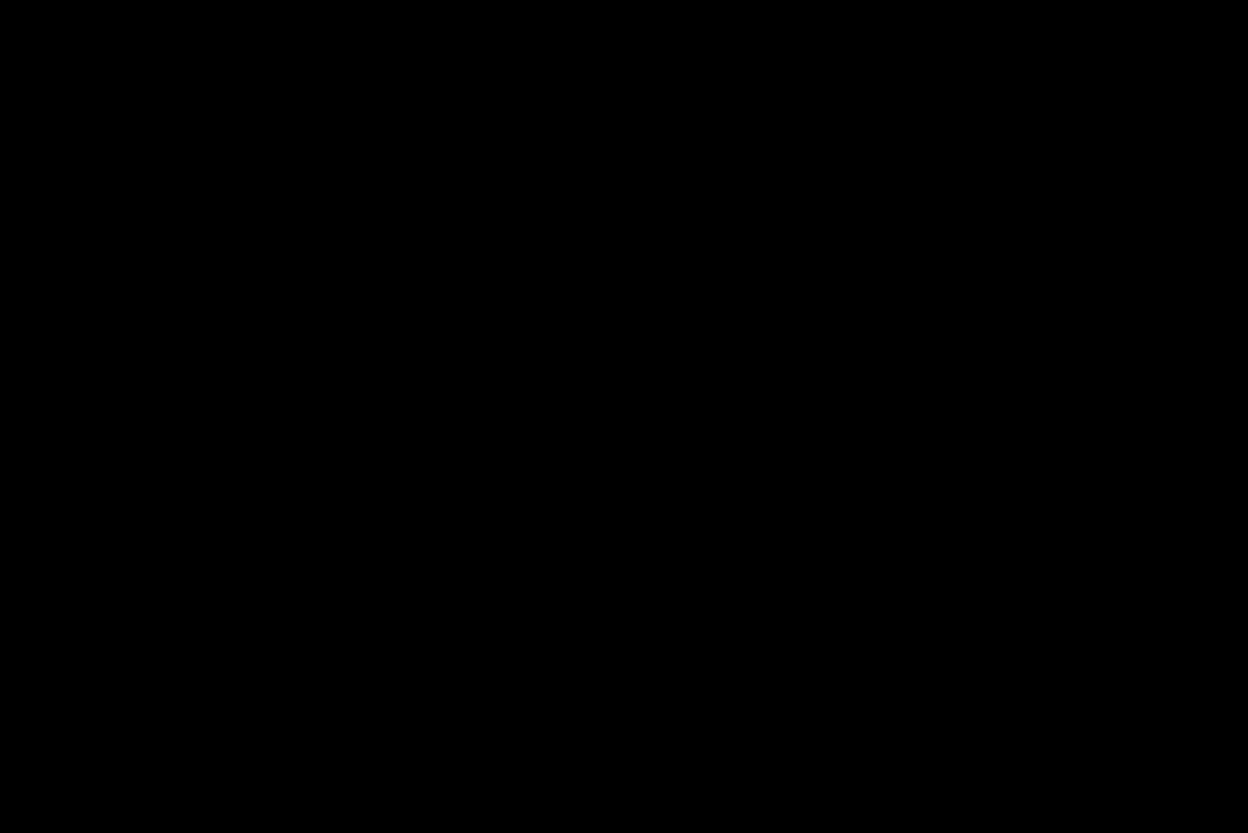
\includegraphics[width=.32\linewidth]{images/Result4/full_odom.jpg}
	}
	\caption{(a), (b), and (c) and (d), (e), and (f) correspond to the 3 x 2 Configuration.}
	
	\label{fig:3_2_Configuration} 
\end{figure*}

\newpage
\section{1-2-1 Configuration}
\begin{figure}[!h] 
	\centering
	\captionsetup[subfigure]{width=.96\linewidth}
	\subfloat[Image 1.]{\label{fig:1_2_1_Configuration_1}
		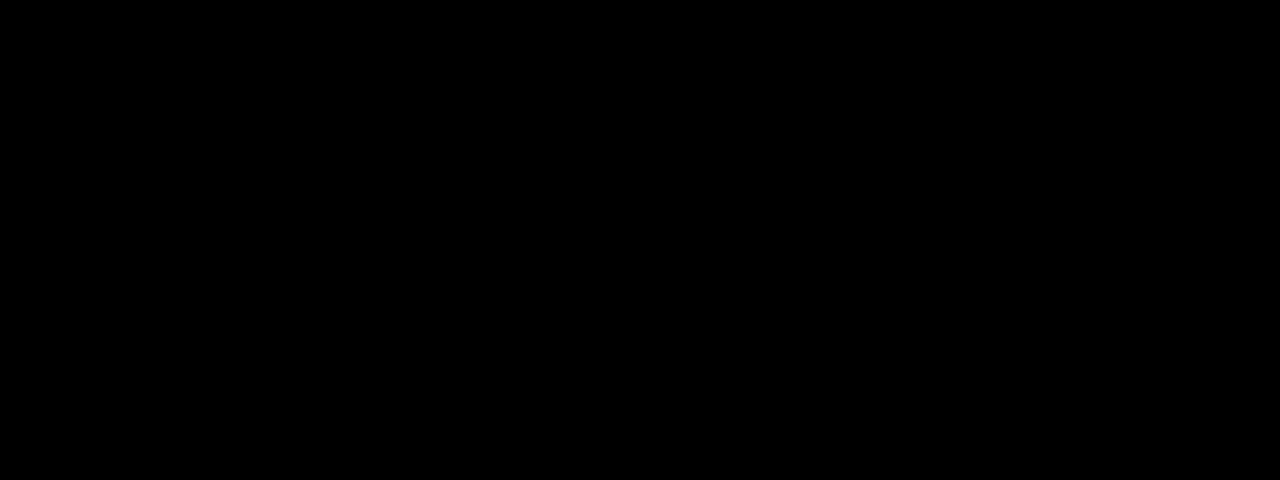
\includegraphics[width=.98\linewidth]{images/Result2/matching.jpg}
	}
	\hfil
	\captionsetup[subfigure]{width=.45\linewidth}
	\subfloat[Image 2.]{\label{fig:1_2_1_Configuration_2}
		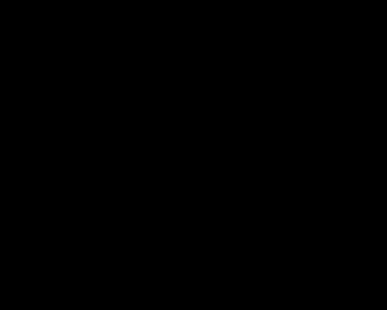
\includegraphics[width=.48\linewidth]{images/Result2/poses.jpg}
	}
	\subfloat[Image 3.]{\label{fig:1_2_1_Configuration_3}
		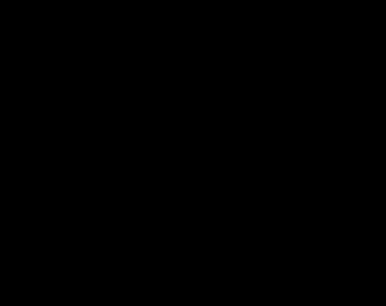
\includegraphics[width=.48\linewidth]{images/Result2/point_SALM.jpg}
	}
	\hfil
	\captionsetup[subfigure]{width=.98\linewidth}
	\subfloat[Image 4.]{\label{fig:1_2_1_Configuration_4}
		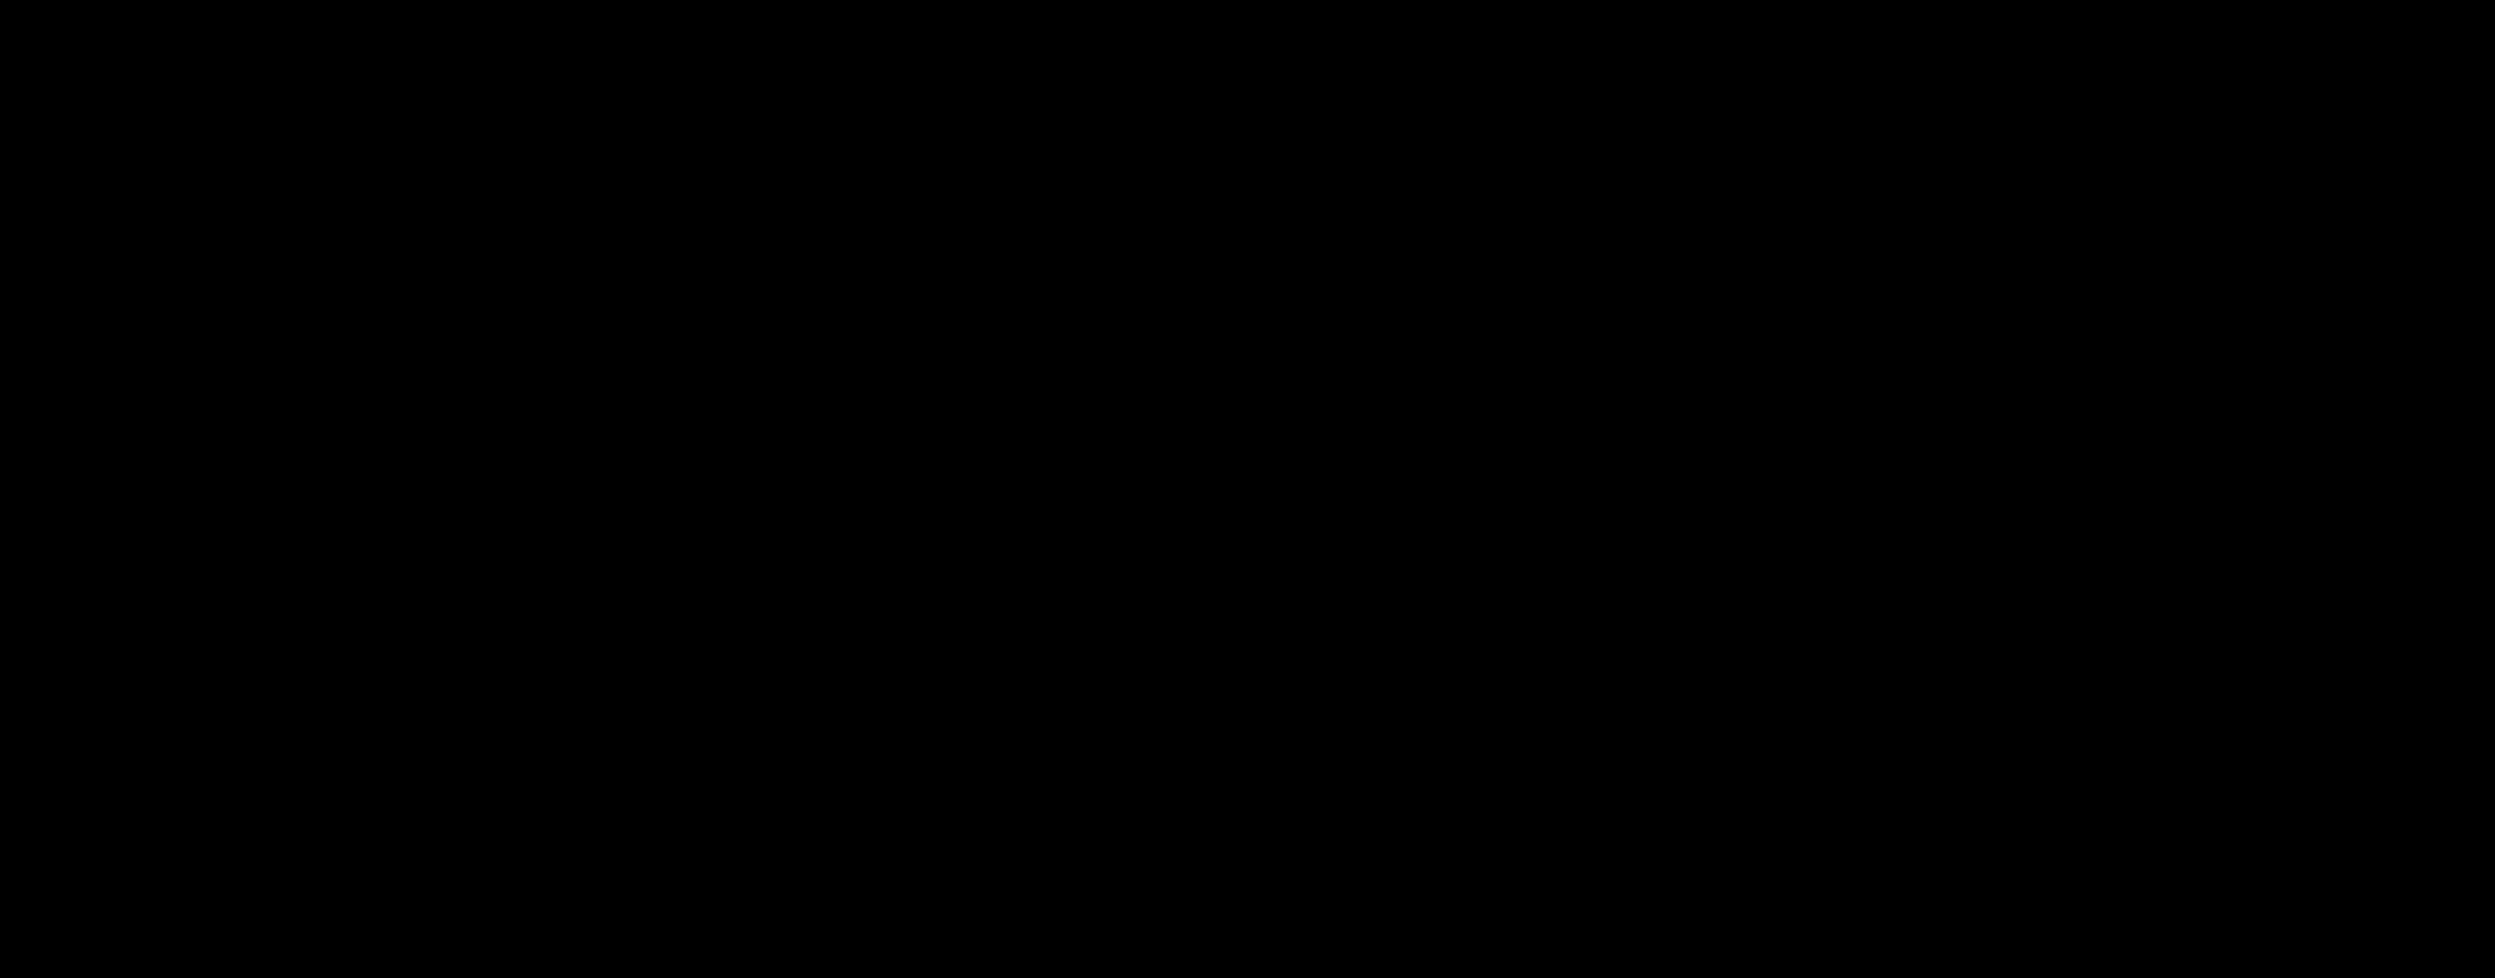
\includegraphics[width=.98\linewidth]{images/Result2/full_map.jpg}
	}
	\caption{\text{1-2-1} Configuration.}
	
	\label{fig:1_2_1_Configuration} 
\end{figure}

\newpage

\section{Appendix}
\label{sec.appen}

\subsection{Appendix subsection}
\label{appen_d}
\subsubsection{Problem definition}

\newpage
\renewcommand*{\bibname}{\section{References}}
\bibliographystyle{ieeetr}
\bibliography{Thesis}

\chapter{Equations and Algorithm}
\label{sec-figures}

\section{Equations and Algorithm}
Let us assume $\gamma_{ij}$ is the number of matched keypoints among two keyframes, $i$ and $j$. These matches yield a distinct scale difference $\sigma_{ij} $ depending on the number of matched keypoints $\gamma_{ij}$. The optimal scale difference $\sigma^*$ will be
\begin{equation}
	\begin{aligned}
		\sigma^* &= \operatorname*{argmax}_{\gamma} \frac{1}{2}|\gamma(\sigma_{ij}), \gamma(\sigma_{i'j'}) | ,
	\end{aligned}
	\label{eqa-1}
\end{equation} 
where $\sigma_{ij} $ and $\sigma_{i'j'}$ are the two nearest points such that\\
\begin{equation}
	\begin{split}
		\quad |\sigma_{ij} - \sigma_{i'j'}| \leq \Delta^* \quad \forall \quad i, j, i' \text{ and } j' \in \mathds{Z}^+, \quad \Delta^* \in \mathbb{R}.
	\end{split}
	\label{eqa-1}
\end{equation} 
The estimation is further explained in Algorithm \ref{algorithm-1}.\\

\begin{algorithm}[!h]
	\SetKwInput{KwData}{Input}
	\SetKwInput{KwResult}{Output}
	\KwData{Matched keyframes $\mathbf{K}_{r_{ID}} = \{\mathbf{K}^i_{s},\mathbf{K}^j_{t}\}$ , poses $^w\mathbf{T}_{r_{ID}} = \{^w\mathbf{T}_{s}, \, ^w\mathbf{T}_{t} \}$, point clouds $P_{r_{ID}}^\mathcal{F} = \{P^{\mathcal{F}_s^i}_{s(i)},P^{\mathcal{F}_t^j}_{t(j)}$\} with $i,j \in \mathds{Z}^+$ }
	\KwResult{Optimal scale difference $\sigma^*$, initial guess relative transformation $^{si}\mathbf{T}_{ti}^{IG}$ }
	initialization\;
	\For{$z = -1:1$} {
		$ P_{s(i+z)}^{\mathcal{F}_w} = \,^w\mathbf{T}_{s(i+z)} (P^{\mathcal{F}_{s(i+z)}}_{s(i+z)}) $ \;
		$ P_{t(j+z)}^{\mathcal{F}_w} = \,^w\mathbf{T}_{t(j+z)} (P^{\mathcal{F}_{t(j+z)}}_{t(j+z)}) $ \;
		\SetKwFunction{FMain}{ PCR-Pro \cite{Bhutta2018}}
		\SetKwProg{Fn}{Function}{:}{}
		\Fn{\FMain{$\mathbf{K}_{r_{ID}}$,$P_{r_{ID}}^{\mathcal{F}_w}$}}{
			Estimate volume ratio $r_{vol}$ of $P_{s(i+z)}^{\mathcal{F}_w}, P_{t(j+z)}^{\mathcal{F}_w}$ \;
			$^{s(i+z)}\mathbf{T}_{t(j+z)}^{RC} \longleftarrow \gamma_z \longleftarrow \mathbf{K}^{i+z}_{s},\mathbf{K}^{j+z}_{t} $ \; 
			$ \sigma_z \longleftarrow ^{s(i+z)}\mathbf{T}_{t(j+z)}^{RC} , \gamma_z, ^w\mathbf{T}_{s(i+z)} , ^w\mathbf{T}_{t(j+z)} $\;
			$^{s(i+z)}\mathbf{T}_{t(j+z)}^{IG} \longleftarrow \sigma_z, P_{s(i+z)}^{\mathcal{F}_w},P_{t(j+z)}^{\mathcal{F}_w} $ \;
			\KwRet $\sigma_z, ^{s(i+z)}\mathbf{T}_{t(j+z)}^{IG} $ \; }
	}
	\eIf{$r_{vol} > 0.5$}{
		$\Delta^* = 5 $\;
		\For{$x = -1: 1$}{
			\For{$y = -1: 1$}{
				\If{$x \neq y$}{
					$ \Delta = |\sigma_x - \sigma_y| $\;
					\If{$\gamma^* < \gamma_{xy}$ \&\& $\Delta^* > \Delta$ \&\& $\Delta^* \neq 0$ }{
						$\sigma^* = avg(\sigma_x,\sigma_y)$ \;
						$\Delta^* = \Delta$ \;
						$\gamma^* = \gamma_{xy}$ \;
					}
				}
			}
		}
	}{ $\sigma^* =\sigma_{xy=00} $ \; } 
	\caption{Finest Tuning for Optimal Scale Estimation}
	\label{algorithm-1}
\end{algorithm}

\newpage

\section{Appendix}

\newpage
\renewcommand*{\bibname}{\section{References}}
\bibliographystyle{ieeetr}
\bibliography{Thesis}	

\chapter{Tabls and Graphs}
\label{sec-pslen}



\section{Table}
Table \ref{table-1} is shown below.

You can also create different style of latex table using link \url{https://www.tablesgenerator.com/}.
\begin{table*}[h]
	\caption{Table I}
	\centering
	\renewcommand{\arraystretch}{1.2}%
	\begin{tabular}{|c|c|c|c|c|}
		\hline
		\multirow{2}{*}{Method}                                   & \multirow{2}{*}{Type} & \multicolumn{3}{c|}{Tested On}                                                                  \\ \cline{3-5}

		                                                          &                       & \multicolumn{1}{c|}{Recall@1}  & \multicolumn{1}{c|}{Recall@5} & \multicolumn{1}{c|}{Recall@10} \\
		\hline
		\hline
		\multirow{2}{*}{Method 1}                                 & Type 1                & 44.76                          & 60.95                         & 70.16                          \\

		                                                          & Type 2                & 52.70                          & 67.30                         & 73.02                          \\
		\hline
		\multirow{2}{*}{Method 2 \cite{arandjelovic2016netvlad} } & Type 1                & 60.00                          & 73.65                         & 79.05                          \\

		                                                          & Type 2                & 58.73                          & 74.6                          & 80.32                          \\
		\hline
		\multirow{2}{*}{Method 3 \cite{zhu2018attention} }        & Type 1                & 61.90                          & 77.78                         & 80.95                          \\

		                                                          & Type 2                & 66.98                          & 80.95                         & 83.81                          \\
		\hline
		Method 4
		                                                          & Type 1                & 66.98                          & 80.95                         & \textbf{85.71}                 \\
		(Ours)                                                    & Type 2                & \textbf{67.30}                 & \textbf{81.27}                & \textbf{85.71}                 \\


		\hline
	\end{tabular}
	\label{table-1}
\end{table*}


\begin{table*}[]
	\centering
	\renewcommand{\arraystretch}{1.5}
	\caption{Table II}
	\label{table-2}
	\begin{tabular}{||c|c|c|cc|cc||}
		\hline
		\multirow{2}{*}{\textbf{Method}} & \multirow{2}{*}{\textbf{Type}} & \multirow{2}{*}{\textbf{Number}} & \multicolumn{2}{c|}{\begin{tabular}[c]{@{}c@{}}\textbf{Total Time} \\ \textbf{Duration (sec)}\end{tabular}} & \multicolumn{2}{c||}{\textbf{Field 3}}                                                         \\ \cline{4-7}
		                                  &                                &                                  & \begin{tabular}[c]{@{}c@{}}
		                                  	Field \\
		                                  	1
		                                  \end{tabular}                      & \begin{tabular}[c]{@{}c@{}}Field \\ 2\end{tabular}            & \begin{tabular}[c]{@{}c@{}}Field 1 \\ Time (sec)\end{tabular} & \begin{tabular}[c]{@{}c@{}}Field \\ 2\end{tabular} \\ \hline \hline
		Method 1                               & Indoor                         & 2                                & 53.7                                           & 69                                   & 0.98                      & 2.4922                    \\ \hline
		\begin{tabular}[c]{@{}c@{}}Method \\ 2\end{tabular}         & Outdoor                        & 2                                & 73                                             & 74                                   & 0.89                      & 2.83519                   \\ \hline
		\begin{tabular}[c]{@{}c@{}}Method 3 \end{tabular}         & Outdoor                        & 2                                & 104                                            & 91                                   & 0.94                      & 1.7857                    \\ \hline
		\begin{tabular}[c]{@{}c@{}}Method 4 \end{tabular}         & \multirow{2}{*}{Outdoor}       & \multirow{2}{*}{3}               & 122                                            & 117                                  & 0.92                      & 1.2786                    \\ \cline{1-1}\cline{4-7}
		\begin{tabular}[c]{@{}c@{}}Method 5 \end{tabular}        &                                &                                  & 122                                            & 112                                  & 0.867                     & 1.15                      \\ \hline
	\end{tabular}%
\end{table*}


\begin{table*}[]
	\centering
	\renewcommand{\arraystretch}{1.5}
	\caption{Table III}
	\label{table-3}
	\begin{tabular}{||c|c|cc|cc|cc||}
		\hline
		\multirow{2}{*}{\textbf{Benchmarks}} & \multirow{2}{*}{\textbf{Direction}} & \multicolumn{2}{c|}{\textbf{Method 1} \cite{Bhutta2018}} & \multicolumn{2}{c|}{\begin{tabular}[c]{@{}c@{}}\textbf{Method} \\ \textbf{2 }\cite{Kummerle2011}\end{tabular}} & \multicolumn{2}{c||}{\textbf{\begin{tabular}[c]{@{}c@{}}Method 3\\ (Proposed)\end{tabular}}}                                                                                        \\ \cline{3-8}
		                                  &                                     & \begin{tabular}[c]{@{}c@{}}Time \\ (sec)\end{tabular}                              & \begin{tabular}[c]{@{}c@{}}RMSE \\ (m)\end{tabular}                      & \begin{tabular}[c]{@{}c@{}}Time \\ (sec)\end{tabular}                                & \begin{tabular}[c]{@{}c@{}}RMSE \\ (m)\end{tabular} & \begin{tabular}[c]{@{}c@{}}Time \\ (sec)\end{tabular} & \begin{tabular}[c]{@{}c@{}}RMSE \\ (m)\end{tabular} \\ \hline \hline
		Benchmark 1                               & Same                                & 7.6                                                     & 0.1503                                          & 5.1                                                       & 0.0903                     & \textbf{2.53}              & \textbf{0.0290}            \\ \hline
		\begin{tabular}[c]{@{}c@{}}Benchmark\\ 2\end{tabular}        & Same                                & 8.8                                                     & 1.2453                                          & 5.5                                                       & 0.9832                     & \textbf{2.93}              & \textbf{0.0323}            \\ \hline
		\begin{tabular}[c]{@{}c@{}}Benchmark 3 \end{tabular}        & Same                                & 7.4                                                     & 1.5594                                          & 5.04                                                      & 0.0883                     & \textbf{2.47}              & \textbf{0.0486}            \\ \hline
		\begin{tabular}[c]{@{}c@{}}Benchmark 4 \end{tabular}        & Opposite                            & 9                                                       & 1.6                                             & 5.57                                                      & 0.207                      & \textbf{3}                 & \textbf{0.175}             \\ \hline
		\begin{tabular}[c]{@{}c@{}}Benchmark 5 \end{tabular}        & Same                                & 11                                                      & 0.3613                                          & 6.24                                                      & 0.3073                     & \textbf{3.67}              & \textbf{0.0712}            \\ \hline
	\end{tabular}%
\end{table*}



\section{Tikz styles Graphs}



\begin{figure}[h]

	\centering
	\raggedright
	\captionsetup[subfigure]{width=.95\linewidth}
	\subfloat[Example 1]
	{	\label{fig:Tikz-1}
		\resizebox{.47\linewidth}{!}{
			\begin{tikzpicture}[trim axis left]%
				\begin{axis}
					[curve plot style]

					\addplot [color=blue, mark=diamond, mark size=3pt, line width=0.8pt]
					table {data/vd16_pitts30k_to_tokyo247_maqbool_DT_50_512.dat};

					\addplot [color=green, mark=square, mark size=3pt, line width=0.8pt]
					table {data/vd16_pitts30k_to_tokyo247_maqbool_DT_100_512.dat};

					\addplot [color=black, mark=asterisk, mark size=3pt, line width=0.8pt]
					table {data/vd16_pitts30k_to_tokyo247_netvlad_512.dat};

					\legend{CURVE-1$_{DT-50}$(ours), CURVE-2$_{DT-100}$(ours),CURVE-3}
				\end{axis}
			\end{tikzpicture}
		}
	}
	\captionsetup[subfigure]{width=.95\linewidth}
	\subfloat[Example 1]
	{\label{fig:Tikz-2}
		\resizebox{.47\linewidth}{!}{

			\pgfplotsset{ymax=90, ymin= 64} %

			\begin{tikzpicture}[trim axis left]%
				\begin{axis}
					[curve plot style]

					\addplot [color=blue, mark=diamond, mark size=3pt, line width=0.8pt]
					table {data/vd16_pitts30k_to_tokyo247_maqbool_DT_50_4096.dat};

					\addplot [color=green, mark=square, mark size=3pt, line width=0.8pt]
					table {data/vd16_pitts30k_to_tokyo247_maqbool_DT_100_4096.dat};

					\addplot [color=black, mark=asterisk, mark size=3pt, line width=0.8pt]
					table {data/vd16_pitts30k_to_tokyo247_netvlad_4096.dat};

					\legend{CURVE-1$_{DT-50}$(ours), CURVE-2$_{DT-100}$(ours),CURVE-3}
				\end{axis}
			\end{tikzpicture}
		}
	}
	\caption{\textbf{Note:} All the curves are in data folders and in `dat' file. Using `\textbf{pgfplotsset}', you can also control the y-axis. `\textbf{tikz\_styles.tex}' has all the further configuration.}
	\label{fig:pitts2tokyo}
\end{figure}


\newpage
\renewcommand*{\bibname}{\section{References}}
\bibliographystyle{ieeetr}
\bibliography{Thesis}


\chapter{Conclusion and Future Work}
\label{sec-conclusion}

Here is conclusion...

\section{Summary of Contributions}



\subsection{Contribution 1}

\subsection{Contribution 1}
\label{maqbool}

\section{Future Work and Challenges}

\subsection{Future Work 1} 

\subsubsection{Part 1} 

\subsubsection{Part 2} 




\end{document}
